\documentclass[12pt,twoside,a4paper]{article}

\usepackage[margin=2cm]{geometry}
\usepackage[slantfont,boldfont]{xeCJK}
\usepackage[utf8]{inputenc}
\usepackage{listings}
\usepackage{float}
\usepackage{color}
\usepackage{xcolor}
\usepackage{caption}
\usepackage{courier}
\usepackage{subfig}

\definecolor{codegreen}{rgb}{0,0.6,0}
\definecolor{codepurple}{rgb}{0.58,0,0.82}
\definecolor{backcolour}{rgb}{0.95,0.95,0.92}
\definecolor{darkgray}{rgb}{0.3,0.3,0.3}

\newcommand{\inlinecode}[1]{\colorbox{backcolour}{\color{darkgray}\texttt{#1}}}

\DeclareCaptionFont{white}{\color{white}}
\DeclareCaptionFormat{listing}{\colorbox{gray}{\parbox{\textwidth}{#1#2#3}}}
\captionsetup[lstlisting]{format=listing,labelfont=white,textfont=white}
\lstset{
	backgroundcolor=\color{backcolour},
	commentstyle=\color{codegreen},
    keywordstyle=\color{violet},
    stringstyle=\color{codepurple},
	language=Python,
	numbers=left,
	numberstyle=\small\color{lightgray},
	columns=fullflexible,
	showstringspaces=false,
	breaklines=true
}

\setCJKmainfont{PingFang TC}

\title{Computer Vision\\Homework 3 Report}
\author{林義聖\\B03902048}
\date{\today}

\usepackage{graphicx}
\graphicspath{ {./} }

\begin{document}

\maketitle

\section{Introduction}

I use \textit{Python} as my programming language and \textit{Pillow} as my Image Library. Also, I use \textit{matplotlib} to draw the histogram.

\section{Histogram Equalization}
I use the following steps to equalize \textit{lena.bmp}.
\begin{enumerate}
	\item Read lena.bmp in as Python \textit{list}.
	\item Loop through every pixels, accumulate its intensity.
	\item Calculate the CDF of its intensity.
	\item Equalize the image using CDF.
\end{enumerate}

\begin{lstlisting}[caption=Equalize the image]
class HistEqualization:
    def __init__(self, data, img_size):
        self.data = data
        self.img_size = img_size
        self.hist_lst = self.calc_histogram()
        self.cdf_lst = self.calc_cdf()

    # accumulate intensity to get histogram
    def calc_histogram(self):
        lst = [0] * 256
        for x in range(self.img_size):
            lst[ self.data[x] ] += 1
        return lst

    # from hist_lst, calculate CDF
    def calc_cdf(self):
        lst = [0] * 256
        for x in range(1,256):
            lst[x] = lst[x-1] + self.hist_lst[x]
        return lst

    # equalize the data
    def equalized(self):
        cdf_min = 0
        lst = [0] * self.img_size
        intensity = [0] * 256

        for x in range(256):
            if self.cdf_lst[x] > 0:
                cdf_min = self.cdf_lst[x]
                break

        for x in range(256):
            if self.cdf_lst[x] < cdf_min:
                intensity[x] = 0
            else:
                intensity[x] = int(round( (float(self.cdf_lst[x] - cdf_min) / float(self.img_size - cdf_min)) * 255.0 ))

        for x in range(self.img_size):
            lst[x] = intensity[ self.data[x] ]

        return lst
\end{lstlisting}

\begin{figure}[H]
\centering
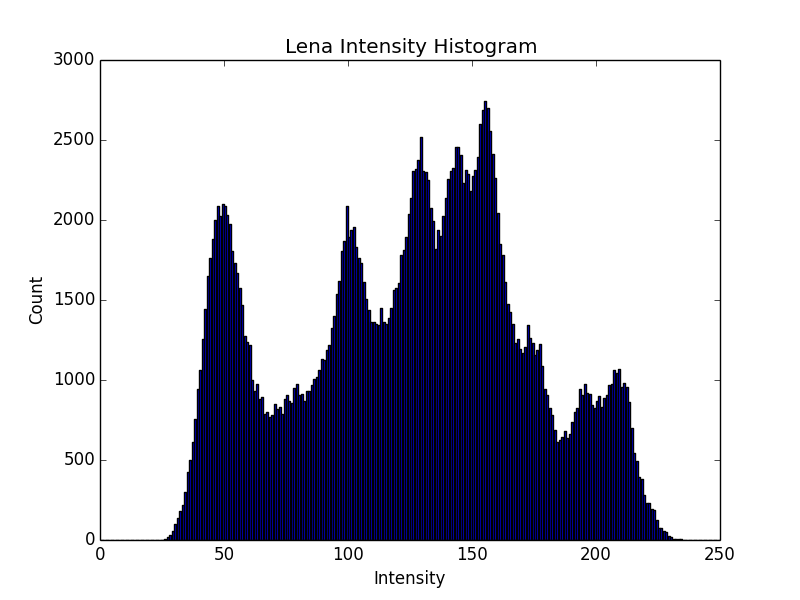
\includegraphics[scale=0.7]{lena-histogram.png}
\caption{original lena histogram}
\label{fig:lena-histogram.png}
\end{figure}

\begin{figure}[H]
\centering
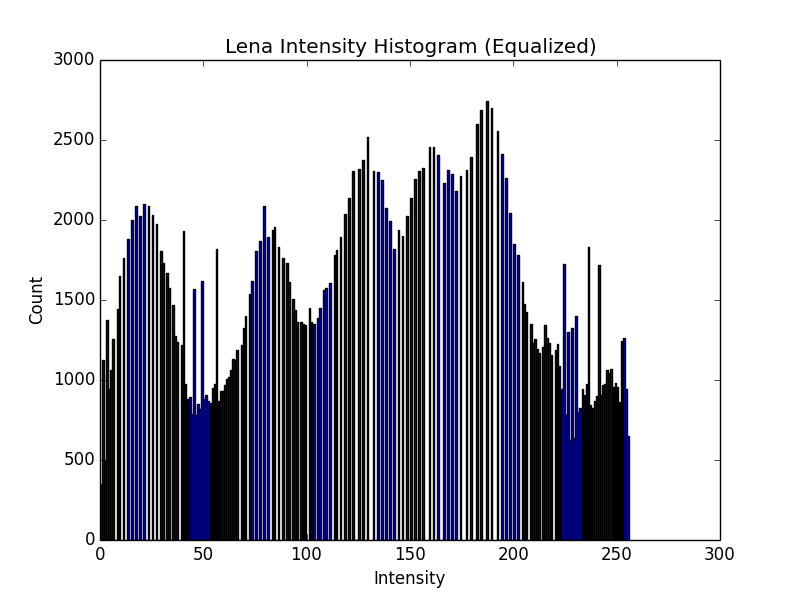
\includegraphics[scale=0.7]{equalized-histogram.png}
\caption{equalized histogram}
\label{fig:equalized-histogram.png}
\end{figure}

\begin{figure}[H]
\centering
\subfloat[original picture] {
    \includegraphics[width=0.45\linewidth]{lena.bmp}
    \label{fig:lena.bmp}
}
\hfill
\subfloat[equalized picture] {
    \includegraphics[width=0.45\linewidth]{lena-equalized.bmp}
    \label{fig:lena-equalized.bmp}
}
\caption{Comparison between two pictures}
\end{figure}

\section{HSV Equalization (additional)}
Additionally, I write the other program to equalize the image. I change the image data from \textit{RGB} mode to \textit{HSV} mode and use the same algorithm but apply on \textit{S - saturation} and \textit{V - lightness}. The program is longer than the previous one. So I won't paste it here, just show the result.

\begin{figure}[H]
\centering
\subfloat[original picture] {
    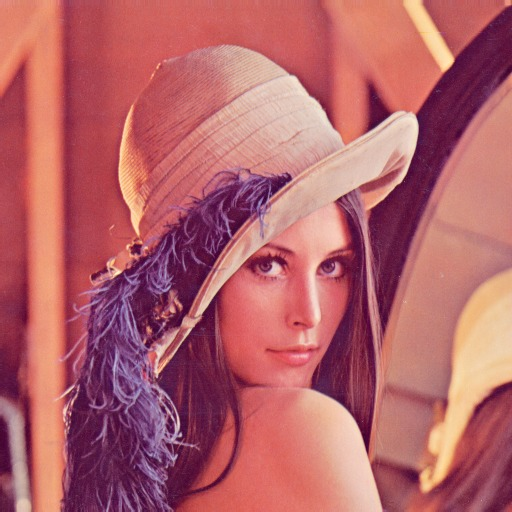
\includegraphics[width=0.45\linewidth]{lena-rgb.jpg}
    \label{fig:lena-rgb.jpg}
}
\hfill
\subfloat[equalized picture] {
    \includegraphics[width=0.45\linewidth]{lena-color.bmp}
    \label{fig:lena-color.bmp}
}
\caption{Comparison between two colorful pictures}
\end{figure}

\section{How to Use}
There are 2 programs,
\begin{enumerate}
    \item \textit{histogram-equalization.py}
    \item \textit{hsv-equalization.py} (additional)
\end{enumerate}
You just need to enter command in this format: "\textit{program [input image name] [output image name]}" to use it. For example, \inlinecode{./histogram-equalization.py lena.bmp output.bmp}.

\end{document}
